\documentclass[11pt]{amsart}

\usepackage[usenames,dvipsnames,svgnames,table]{xcolor}
\usepackage[colorlinks=true, pdfstartview=FitV, linkcolor=blue, citecolor=blue, urlcolor=darkblue]{hyperref}

%\usepackage{addfont}
%\addfont{OT1}{rsfs10}{\rsfs}

\usepackage{geometry}                % See geometry.pdf to learn the layout options. There are lots.
\geometry{letterpaper}                   % ... or a4paper or a5paper or ...
%\geometry{landscape}                % Activate for for rotated page geometry
%\usepackage[parfill]{parskip}    % Activate to begin paragraphs with an empty line rather than an indent
\usepackage{graphicx}
\usepackage{mathrsfs}
\usepackage{amssymb}
\usepackage{amsfonts}
\usepackage{mathrsfs}
\usepackage{epstopdf}
\usepackage{lscape}
\usepackage[utf8]{inputenc}
\usepackage{tikz,caption}
\DeclareGraphicsRule{.tif}{png}{.png}{`convert #1 `dirname #1`/`basename #1 .tif`.png}
\usepackage{enumitem}
\setlist[itemize]{leftmargin=2em}
\setlist[enumerate]{leftmargin=2em}
\usepackage{booktabs}
\usepackage{multirow}
\usepackage{mathtools}
\usepackage[linesnumbered,ruled]{algorithm2e}

\definecolor{darkblue}{rgb}{0.0,0,0.7} % darkblue color
\definecolor{darkred}{rgb}{0.7,0,0} % darkred color
\definecolor{darkgreen}{rgb}{0, .6, 0} % darkgreen color

% Dark red emphasis
\newcommand{\defncolor}{\color{darkred}}
\newcommand{\defn}[1]{{\defncolor\emph{#1}}} % emphasis of a definition

\newtheorem{theorem}{Theorem}[section]
\newtheorem{prop}[theorem]{Proposition}
\newtheorem{cor}[theorem]{Corollary}
\newtheorem{lemma}[theorem]{Lemma}
\newtheorem{conj}[theorem]{Conjecture}
\theoremstyle{definition}
\newtheorem{definition}[theorem]{Definition}
\newtheorem{example}[theorem]{Example}
\newtheorem{remark}[theorem]{Remark}
\numberwithin{equation}{section}

\usepackage[colorinlistoftodos]{todonotes}
\newcommand{\idiot}[1]{\vspace{5 mm}\par \noindent
\marginpar{\textsc{Note}}
\framebox{\begin{minipage}[c]{0.95 \textwidth}
#1 \end{minipage}}\vspace{5 mm}\par}
\newcommand{\mike}[1]{\todo[size=\tiny,color=lime!30]{#1 \\ \hfill --- Mike}}
\newcommand{\nantel}[1]{\todo[size=\tiny,color=red!30]{#1 \\ \hfill --- Nantel}}
\newcommand{\yohana}[1]{\todo[size=\tiny,color=Cyan]{#1 \\ \hfill --- Yohana}}
\newcommand{\farad}[2][]{\todo[size=\tiny,color=ForestGreen!30,#1]{#2 \\ \hfill --- Farad}}
\newcommand{\kelvin}[1]{\todo[size=\tiny,color=RoyalBlue!30]{#1 \\ \hfill --- Kel}}

%remove the comment from the following line to remove all the
% extra proofs:
%\renewcommand{\idiot}[1]{}

\title{Quasi-symmetric harmonics of the exterior algebra}
\author{Nantel Bergeron,
Kelvin Chan,
Yohana Solomon,
Farhad Soltani,
Mike Zabrocki}
\date{Draft November 2021}

\begin{document}

\maketitle

\section{Introduction}

\section{Quasisymmetric invariants on the exterior algebra}

Fix $n$ a positive integer and
let $R_n = {\mathbb Q}[\theta_1, \theta_2, \ldots, \theta_n]$ be the
polynomial ring in anticommuting variables.
The ring $R_n$ is isomorphic to the exterior algebra of a vector
space of dimension $n$.  The variables of this ring satisfy the relations
\[
\theta_i \theta_j = - \theta_j \theta_i \hbox{ if } 1 \leq i \neq j \leq n
\qquad\hbox{and}\qquad \theta_i^2 = 0 \hbox{ for }1 \leq i \leq n~.
\]
Since these conditions impose that a monomial in $R_n$ has no repeated variables,
the monomials are in bijection with subsets of $\{1,2,\ldots, n\}$
and the dimension of $R_n$ is therefore equal to $2^n$.

Denote $[n] := \{1,2, \ldots,n\}$ and
let $A = \{a_1 < a_2 < \cdots < a_r \} \subseteq [n]$.
We define $\theta_A := \theta_{a_1} \theta_{a_2} \cdots \theta_{a_r}$,
then the set $\{ \theta_A \}_{A \subseteq [n]}$ is a basis of $R_n$.

We define an action on monomials of $R_n$ and extend this action linearly.
For each integer $1 \leq i < n$, let $\pi_i$ be an operator on $R_n$
that is defined by
\[
\pi_i(\theta_A) = \begin{cases}
\theta_{A} & \hbox{ if } i, i+1 \in A\hbox{ or }i, i+1 \notin A\\
\theta_{A \cup \{i+1\} \backslash \{i\}} & \hbox{ if } i\in A\hbox{ and }i+1 \notin A\\
\theta_{A \cup \{i\} \backslash \{i+1\}} & \hbox{ if } i+1\in A\hbox{ and }i \notin A
\end{cases}~.
\]
These operators instead of exchanging an $i$ for an $i+1$ like the symmetric group
action, have the effect of shifting the indices of the variables (if possible).  They
are therefore known as quasisymmetric operators.  They were studied in depth by
Hivert \cite{H}.  The operators are not multiplicative on $R_n$ in general since, for example,
\[
\pi_1( \theta_{1} \theta_{2})
= \theta_1 \theta_2
= - \pi_1( \theta_{1}) \pi_1(\theta_{2})~.
\]
They are also not multiplicative when they act on the polynomial ring
in commuting variables.

A polynomial that is invariant under the action of quasisymmetric operators
is said to be quasisymmetric invariant (or just `quasisymmetric').
The quasisymmetric invariants of $R_n$ are
linearly spanned by the elements:
\begin{equation}\label{eq:defF}
F_{1^r}(\theta_1, \theta_2, \ldots, \theta_n) := \sum_{\substack{A \subseteq [n]\\|A|=r}} \theta_A~.
\end{equation}
The notation $F_{1^r}$ for the elements borrow the notation from the
polynomial ring in commuting variable invariants known as the `fundamental
quasisymmetric polynomials'.  The commuting polynomial quasisymmetric
invariants are indexed by compositions.

\begin{remark}
As expressing polynomials with listing the variables
(e.g. $p(\theta_1, \theta_2, \ldots, \theta_n)$) can be notational cumbersome
there will be points where we will drop the variables in the expressions
and this will is to indicate that the polynomials are in the
variables $\theta_1, \theta_2, \ldots, \theta_n$.  There will also
be expressions where some polynomials have fewer variables and there
we will indicate this by listing the variables.
\end{remark}

\subsection{The ideal generated by the quasisymmetric invariants}

Define an ideal of $R_n$ generated by the quasisymmetric invariants as
\[
I_n := \left< F_{1^r}(\theta_1, \theta_2, \ldots, \theta_n) : 1 \leq r \leq n \right>
\]

\begin{remark}
Note that since the operators $\pi_i$ are not multiplicative, it
is unlikely to be the case that $I_n$ as an ideal is invariant
under the action of the $\pi_i$.  Indeed, we find that for $n=4$,
\[
\theta_2 F_{1}(\theta_1, \theta_2, \theta_3, \theta_4) =
-\theta_1 \theta_2 + \theta_2 \theta_3 + \theta_2 \theta_4
\]
and if we apply $\pi_1$ to this element, we obtain
\[
\pi_1(\theta_2 F_{1}(\theta_1, \theta_2, \theta_3, \theta_4)) =
-\theta_1 \theta_2 + \theta_1 \theta_3 + \theta_1 \theta_4
\]
and this can be shown to not be in $I_4$.
\end{remark}

The \emph{exterior quasisymmetric coinvariants} are defined to be
\mike{I hesitated to give a three letter abbreviated name, like EQC,
but I don't know a better way to
capture the `anti-commuting' and the `quasisymmetric' and the
`coinvariants' in just two letters}
\nantel{and is it really coinvariant? (since the ideal is not invariant)}
\[
EQC_n := R_n/I_n~.
\]

\subsection{Differential operators on the exerior algebra}
We can define a set of differential operators on $R_n$ which
will permit us to define the orthogonal complement to the
ideal and a notion of quasisymmetric harmonics.

The operators $\partial_{\theta_i}$ act on monomials in $R_n$
by
\[
\partial_{\theta_i}( \theta_A ) = \begin{cases}
(-1)^{\#\{ j \in A: j<i\}}\theta_{A \backslash \{i\}}&\hbox{ if }i \in A\\
0&\hbox{ if }i \in A
\end{cases}~.
\]

The operators can equally be characterized by their commutation
relations
\[
\partial_{\theta_i} \partial_{\theta_j}=-\partial_{\theta_j} \partial_{\theta_i}
\hbox{ if } 1 \leq i \neq j \leq n
\qquad\hbox{and}\qquad
\partial_{\theta_i}^2 = 0\hbox{ for }1 \leq i \leq n
\]
\[
\partial_{\theta_i} \theta_j=-\theta_j \partial_{\theta_i}
\hbox{ if } 1 \leq i \neq j \leq n
\qquad\hbox{and}\qquad
\partial_{\theta_i} \theta_i = 1\hbox{ for }1 \leq i \leq n~.
\]

For a monomial $\theta_A = \theta_{a_1} \theta_{a_2} \cdots \theta_{a_r}$,
let $\overline{\theta_A} = \theta_{a_r} \theta_{a_{r-1}} \cdots \theta_{a_1}$ represent the
reversing the order of the variables.  Extend this notation to both
differential operators and polynomials (and polynomials on differential operators)
by extending the notation linearly.

We can define an inner product on $R_n$ by setting for $p,q \in R_n$.
\[
\left< p, q \right> = \overline{p(\partial_{\theta_1}, \partial_{\theta_2}, \ldots, \partial_{\theta_n})}
q( \theta_1, \theta_2, \ldots, \theta_n)|_{\theta_1=\theta_2 = \ldots=\theta_n=0}~.
\]
The monomials of $R_n$ form an orthonormal basis of the space with respect to this
inner product.

Define the orthogonal complement to $I_n$ with respect to the inner product as
the set
\begin{align*}
EQH_n :&= \left\{ q \in R_n : \left< p, q \right> = 0 \hbox{ for all } p \in I_n \right\}\\
  &=\left\{ q \in R_n :\overline{p(\partial_{\theta_1}, \partial_{\theta_2}, \ldots, \partial_{\theta_n})}
q= 0 \hbox{ for all } p \in I_n \right\}~.
\end{align*}
The second equality follows from the fact that $I_n$ is an ideal and show that $EQH_n$ is also the solution space of 
a system of differential equations. We refer to this space as the \emph{exterior quasisymmetric harmonics}.\footnote{
The harmonics and diagonal harmonics borrows the name from the physics literature
because the harmonic operator $\partial_1^2 + \partial_2^2 + \cdots + \partial_n^2$
is symmetric in the differential operators.  In the case of the exterior algebra,
this operator acts as zero and yet we persist by borrowing the name from the
analogous spaces of commuting variables.
}

\begin{prop} For all $n \geq 1$, as graded vector spaces
\[
EQC_n \simeq EQH_n~.
\]\mike{is there a collection of Temperley-Lieb operators for which these spaces are modules and isomorphic?}
\end{prop}
\nantel{We can find a basis of EQC that is closed under Hivert action (without the quotient). Since I don't know anymore what is EQH
I can't tell}

\section{A linear basis of the ring}

Again let $n$ be a fixed positive integer and $R_n = {\mathbb Q}[\theta_1, \theta_2, \ldots, \theta_n]$.
We have thus far represented the basis for
$R_n$ as the elements $\theta_A$ with $A \subseteq [n]$.  Define $\alpha(A) \in \{ 0,1\}^n$ to be
the sequence $a_1 a_2 a_3 \cdots a_n$ with $a_i = 1$ if $i \in A$ and
$a_i = 0$ if $i \notin A$ so that
\[
\theta_A = \theta_1^{a_1} \theta_2^{a_2} \cdots \theta_n^{a_n} := \theta^{\alpha(A)}~.
\]
For such a sequence $\alpha \in \{0,1\}^n$, let $m_1(\alpha) := \sum_{i=1}^n a_i$
represent the number of $1$s in the string.  This will also be the degree of the monomial
$\theta^{\alpha}$.

For sequences $\alpha \in \{ 0, 1 \}^n$, define elements $G_\alpha$ by
\begin{equation}\label{eq:Gdef1}
G_{1^s0^{n-s}} = F_{1^s}
\end{equation}
and if $\alpha \neq 1^s 0^{n-s}$, then $\alpha$ is of the form $u01^s0^{n-k-s}$ for some string $u$
of length $k-1$ and we recursively define
\begin{equation}\label{eq:Gdef2}
G_{u01^s0^{n-k-s}} = G_{u1^s0^{n-k-s+1}} - (-1)^{m_1(u)} \theta_k G_{u1^{s-1}0^{n-k-s+2}}~.
\end{equation}

We will show below that the recurrence for the
$G_\alpha$ are defined so that they are $S$-polynomials \cite{CLO}
for elements of the ideal $I_n$.
In commutative variables, similar polynomials were defined by Aval-Bergeron-Bergeron~\cite{AB,ABB} 
as a (complete) subset of $S$-polynomials needed to compute all possible
$S$-polynomials in the Buchburger algorithm for Gr\"obner basis.
It is not given that one can describe easily such a set of $S$-polynomials and here we have adapted
the definition for working in the exterior algebra.

\begin{example} For $\alpha = 010110$ and $\beta = 001100$, we compute
the elements $G_\alpha$ and $G_\beta$ using the definition.
\begin{align*}
G_{010110} &= G_{011100} + \theta_3 G_{011000} = (G_{111000} - \theta_1 G_{110000})
+ \theta_3(G_{110000} - \theta_1 G_{100000})\\
&= \theta_2 \theta_4 \theta_5 + \theta_2 \theta_4 \theta_6 + \theta_2 \theta_5 \theta_6
+ 2 \theta_3 \theta_4 \theta_5 + 2 \theta_3 \theta_4 \theta_6 + 2 \theta_3 \theta_5 \theta_6
+ \theta_4 \theta_5 \theta_6
\end{align*}

and we have that
\begin{align*}
G_{001100} &= G_{011000} - \theta_2 G_{010000} = (G_{110000} - \theta_1 G_{100000})
- \theta_2 (G_{100000} - \theta_1 G_{000000})\\
&= \theta_3 \theta_4 + \theta_3 \theta_5 + \theta_3 \theta_6 + \theta_4 \theta_5 + \theta_4 \theta_6 + \theta_5 \theta_6
\end{align*}
\end{example}

Order the monomials of $R_n$ so that we say $\theta_A < \theta_B$ if
$\alpha(A)$ is smaller than $\alpha(B)$ in lexicographic order.
An important property of these elements is the following statement.

\begin{prop}
The leading term of $G_\alpha$ is $\theta^\alpha$.
\end{prop}

In order to prove this proposition, we will first establish a lemma.
This lemma is analogous to Lemma 3.3 of \cite{AB}.
The recursion in this lemma is really the origin of the definition
of $G_\alpha$ because Equation \eqref{eq:Gdef2}
was adapted so that this lemma holds.

\begin{lemma}\label{lem:LT}
 Let $\alpha \in \{0,1\}^{n-1}$, then
\begin{align*}
G_{0\alpha} &= G_\alpha(\theta_2, \theta_3, \ldots, \theta_n)\\
\hbox{and }G_{1\alpha} &= \theta_1 G_{0\alpha} + P_{\alpha}(\theta_2, \theta_3, \ldots, \theta_n)\,.
\end{align*}
\end{lemma}
\nantel{I realize we should really index $P$ with $\alpha$ only, this is more coherent with our notation}

\begin{remark}\label{rem:shift}
 By convention, the length of the index for our polynomials indicate in which polynomial space we are.
For example if $\beta   \in \{0,1\}^{n}$ then $G_\beta\in R_n$. For $\alpha \in \{0,1\}^{n-1}$  in Lemma~\ref{lem:LT}, when we write
$G_\alpha(\theta_2, \theta_3, \ldots, \theta_n)$ we mean $G_\alpha\in  R_{n-1}$ inbeded in $R_n$ with the substitution  
$\theta_i:=\theta_{i+1}$. Similarly for $P_\alpha$.
\end{remark}

\begin{proof}[Proof of Lemma~\ref{lem:LT}]
The proof will be by induction on $n-i$ where $i$ is the number of trailing $0$.
The base case $0=n-n$ with $n$ zeros, is $0\alpha = 0^n$ and we have
\[
G_{0^n} = F_{1^0}(\theta_1,\theta_2 ,\ldots,\theta_n) = 1 = G_{0^{n-1}}(\theta_2, \theta_3, \ldots, \theta_n)
\]
We then consider the case  $0\alpha=01^s0^{n-s-1}$. The polynomials $F_{1^s}$ satisfy the  following identity
\begin{equation}\label{eq:relF}
F_{1^s}(\theta_1,\theta_2 ,\ldots,\theta_n) = \theta_1 F_{1^{s-1}}(\theta_2 ,\ldots,\theta_n) + F_{1^s}(\theta_2,\theta_3 ,\ldots,\theta_n)
\end{equation}
This follows directly from the definition~\eqref{eq:defF} where we split the sum in two parts depending if $1\in A$ or not.
The definition of $G_{01^s0^{n-s-1}}$  gives us
\begin{align*}
	G_{01^s0^{n-s-1}}&= G_{1^s0^{n-s}} - \theta_1 G_{1^{s-1}0^{n-s+1}}
	  =F_{1^s}(\theta_1,\theta_2 ,\ldots,\theta_n) - \theta_1 F_{1^{s-1}}(\theta_2 ,\ldots,\theta_n) \\
	  &= F_{1^s}(\theta_2,\theta_3 ,\ldots,\theta_n)= G_{\alpha}(\theta_2,\theta_3 ,\ldots,\theta_n)\,.
\end{align*}
Now lets assume that $0\alpha\ne 01^s0^{n-s-1}$. Therefore $0\alpha=0w01^s0^{n-k-s}$ for some string $w$
of length $k-2$. For $0\alpha=0w01^s0^{n-k-s}$,  we have $n-k-s$ trailing zeros and $n-n+k+s=k+s$. Remark that for $0w1^s0^{n-k-s+1}$
and $0w1^{s-1}0^{n-k-s+2}$ we have more trailing zeros than $0\alpha$ and we will  use the Induction Hypothesis in the
equality~\eqref{eq:IH0}  below.
\begin{align}
	G&_{0w01^s0^{n-k-s}}= G_{0w1^s0^{n-k-s+1}} - \theta_k G_{0w1^{s-1}0^{n-k-s+2}} \nonumber \\ 
	 & = G_{w1^s0^{n-k-s+1}}(\theta_2,\theta_3 ,\ldots,\theta_n) - (-1)^{m_1(0w)} \theta_k G_{w1^{s-1}0^{n-k-s+2}}(\theta_2,\theta_3 ,\ldots,\theta_n) \label{eq:IH0}\\
	 & = \big[G_{w1^s0^{n-k-s+1}} -  (-1)^{m_1(w)} \theta_{k-1} G_{w1^{s-1}0^{n-k-s+2}}\big](\theta_2,\theta_3 ,\ldots,\theta_n)\label{eq:detail0}\\
	 & = G_{w01^s0^{n-k-s+1}} (\theta_2,\theta_3 ,\ldots,\theta_n) = G_{\alpha} (\theta_2,\theta_3 ,\ldots,\theta_n)  \label{eq:final0} 
\end{align}
In~\eqref{eq:detail0} the expression inside the square bracket $[\cdots]$ is as polynomials in the variables $\theta_1,\ldots,\theta_{n-1}$ in $R_{n-1}$ (see Remark~\ref{rem:shift}).
Hence, the variable $\theta_{k}$ has to be replaced by $\theta_{k-1}$. Also, $m_1(0w)=m_1(w)$. The expression we get is exactly the definition of 
$G_{w01^s0^{n-k-s+1}} \in R_{n-1}$ and the equation~\eqref{eq:final0} follows. This conclude the proof of the first equality in the Lemma.

Now we assume that we have $1\alpha=1^{s+1}0^{n-s-1}$.
\end{proof}

The second case is when $\alpha = 01^s0^{n-s-1}$ for $s>0$, then
\[
G_{01^s0^{n-s-1}} = G_{1^s0^{n-s}} - \theta_1 G_{1^{s-1}0^{n-s+1}}
\]
Since $G_{1^s0^{n-s}} = F_{1^s}$ and $G_{1^{s-1}0^{n-s+1}} = F_{1^{s-1}}$
by Equation \eqref{eq:Gdef1}, then since $\theta_1^2 = 0$, we have that
$\theta_1 F_{1^{s-1}}$ is the
sum over all monomials $\theta_A$ where $A \subseteq [n]$ with $|A| = s$ and $1 \in A$.
The difference $F_{1^s} - \theta_1 F_{1^{s-1}}$
is then equal to the sum over all monomials $\theta_A$ where
$A \subseteq [n]$ with $|A| = s$ and $1 \notin A$
and this is equal to $F_{1^s}(\theta_2, \theta_3, \ldots, \theta_n) = G_{1^s0^{n-s-1}}(\theta_2, \theta_3, \ldots, \theta_n)$ again by Equation \eqref{eq:Gdef1}.

Next we prove $G_{0\alpha} = G_\alpha(\theta_2, \theta_3, \ldots, \theta_n)$ by induction
on $k = \ell(w)+1$ and $\alpha = w01^s0^{n-k-s-1}$ for some $s>0$.  Then by Equation
\eqref{eq:Gdef2} and the inductive hypothesis,
\begin{align*}
G_{0w01^s0^{n-k-s-1}} &= G_{0w1^s0^{n-k-s+1}} - (-1)^{m_1(w)} \theta_k G_{0w1^{s-1}0^{n-k-s+2}}\\
&= G_{w1^s0^{n-k-s+1}}(\theta_2, \theta_3, \ldots, \theta_n) -
(-1)^{m_1(w)} \theta_k G_{w1^{s-1}0^{n-k-s+2}}(\theta_2, \theta_3, \ldots, \theta_n)~.
\end{align*}
Now we view $\theta_k G_{w1^{s-1}0^{n-k-s+2}}(\theta_2, \theta_3, \ldots, \theta_n)=
(\theta_{k-1} G_{w1^{s-1}0^{n-k-s+2}})(\theta_2, \theta_3, \ldots, \theta_n)$
and $G_{w1^s0^{n-k-s+1}} - (-1)^{m_1(w)} \theta_{k-1} G_{w1^{s-1}0^{n-k-s+2}} =
G_{w01^s0^{n-k-s+1}}$ by Equation \eqref{eq:Gdef2}.  Therefore,
\[
G_{0w01^s0^{n-k-s-1}} = G_{w01^s0^{n-k-s+1}}(\theta_2, \theta_3, \ldots, \theta_n)
\]
and we see that Equation \eqref{eq:0start} holds by induction.

We next prove Equation \eqref{eq:1start} by induction.  The base case is if $\alpha = 1^s0^{n-s-1}$,
then using Equation \eqref{eq:0start} we have
\begin{align*}
G_{1^{s+1}0^{n-s-1}} &= F_{1^{s+1}} = \theta_1 F_{1^s} + F_{1^{s+1}}(\theta_2, \theta_3, \ldots, \theta_n)\\
&= \theta_1 F_{1^s}(\theta_2, \theta_3, \ldots, \theta_n) + F_{1^{s+1}}(\theta_2, \theta_3, \ldots, \theta_n)
&= \theta_1 G_{01^s0^{n-s-1}} + F_{1^{s+1}}(\theta_2, \theta_3, \ldots, \theta_n)~.
\end{align*}
This shows that \eqref{eq:1start} holds in the case if we let
$P_{1^{s+1}0^{n-s-1}}(\theta_2, \theta_3, \ldots, \theta_n)
= F_{1^{s+1}}(\theta_2, \theta_3, \ldots, \theta_n)$.


\section{A path model for the quotient}

To each sequence $\alpha \in \{0, 1\}^n$, we associate a path starting at the origin
and extending into the first quadrant of the $x,y$-plane.  The $i^{th}$ step of this
path will be in the $(1,0)$-direction if $a_i =1$ and it will be in the $(0,1)$-direction
if $a_i = 0$.  We say that the sequence $\alpha$ \defn{crosses the diagonal} if
there is a point on the path which lies at $(a,a)$ and the next step is in the $(0,1)$
direction.  Otherwise we say that $\alpha$ \defn{stays above the diagonal}.  Note that
$\alpha$ stays above the diagonal if $\sum_{i=1}^r a_i \leq \lfloor r/2 \rfloor$ for all $1 \leq r \leq n$
and it crosses the diagonal otherwise.

\begin{example} Let $n=6$ and $\alpha = 010110$ and $\beta = 001100$, then the corresponding
paths are
\begin{center}
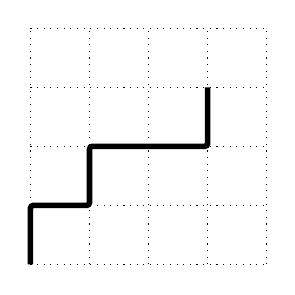
\begin{tikzpicture}[scale=.75]
  \draw[dotted] (0, 0) grid (4, 4);
  \draw[rounded corners=1, color=black, line width=2] (0, 0) -- (0, 1) -- (1, 1) -- (1, 2) -- (2, 2) -- (3, 2) -- (3, 3);
\end{tikzpicture}
\hskip .5in
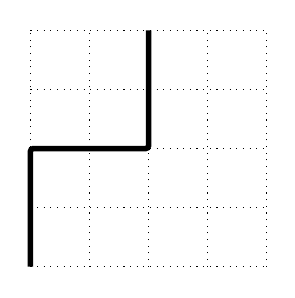
\begin{tikzpicture}[scale=.75]
  \draw[dotted] (0, 0) grid (4, 4);
  \draw[rounded corners=1, color=black, line width=2] (0, 0) -- (0, 1) -- (0, 2) -- (1, 2) -- (2, 2) -- (2, 3) -- (2, 4);
\end{tikzpicture}
\end{center}
\end{example}

The elements $G_\alpha$ are defined so that we could use them to
identify a nice basis of the ideal $I_n$.

\begin{theorem}
If $\alpha$ crosses the diagonal, then $G_\alpha \in I_n$.
\end{theorem}


\begin{thebibliography}{999}
\bibitem{AB} J. C. Aval, N. Bergeron,
\textit{Catalan paths and quasi-symmetric functions}.
Proc. of the Am. Math. Soc., 2003, 131(4), pp. 1053--1062.
\href{https://doi.org/10.1090/S0002-9939-02-06634-0}{10.1090/S0002-9939-02-06634-0}.

\bibitem{ABB} J. C. Aval, F. Bergeron, N. Bergeron,
\textit{Ideals of quasi-symmetric functions and super-covariant polynomials for $S_n$}.
Adv. in Math., 2004, Jan 30, 181 (2), pp. 353--367.
\href{https://doi.org/10.1016/S0001-8708(03)00068-9}{10.1016/S0001-8708(03)00068-9}.

\bibitem{CLO} D. Cox, J. Little, D. OShea,
\textit{Ideals, varieties, and algorithms: an introduction to computational
algebraic geometry and commutative algebra}.
Springer Science \& Business Media; 2013 Mar 9.

\bibitem{H} F. Hivert, 
\textit{Hecke algebras, difference operators, and quasi-symmetric
              functions}.
Adv. in Math., 2000, 155 (2), pp. 181--238.
\href{https://doi-org/10.1006/aima.1999.1901}{10.1006/aima.1999.1901}.

\bibitem{L} S. X. Li,
\textit{Ideals and quotients of diagonally quasi-symmetric functions}.
Elec. J. Comb., Vol 24, Issue \#3, P3.3.
\href{https://doi.org/10.37236/6658}{10.37236/6658}.
\end{thebibliography}

\end{document}


